
\documentclass[11pt,a4paper,UTF8]{book}

\usepackage{minted}
\usepackage[T1]{fontenc}
\usepackage[utf8]{inputenc}
\usepackage{authblk}

\usepackage{fontspec}                  %引入字体设置宏包
\setmainfont{Times New Roman}             %设置英文正文字体
% Courier New
% Book Antique
\setsansfont{Arial}                    %英文无衬线字体
\setmonofont{Courier New}              %英文等宽字体

\usepackage{ctex} %导入中文包
%\usepackage{ulem}
\usepackage{tocvsec2}
\usepackage{verbatim}

\usepackage{tabularx}
\usepackage{longtable}
\usepackage{booktabs}
\usepackage{multirow}
\usepackage{bbding}
\usepackage{float}
\usepackage{xspace}
\usepackage[none]{hyphenat}

\usepackage{graphicx}
\usepackage{subfigure}
\usepackage{pifont}

\usepackage{hyperref}  %制作pdf的目录
\usepackage{subfiles} %使用多文件方式进行

\usepackage{geometry} %设置页边距的包
\geometry{left=2.5cm,right=2cm,top=2.54cm,bottom=2.54cm} %设置书籍的页边距

\usepackage{url}
\hypersetup{hidelinks, %去红框
  colorlinks=true,
  allcolors=black,
  pdfstartview=Fit,
  breaklinks=true
}

% 调整itemlist中的行间距
\usepackage{enumitem}
\setenumerate[1]{itemsep=0pt,partopsep=0pt,parsep=\parskip,topsep=5pt}
\setitemize[1]{itemsep=0pt,partopsep=0pt,parsep=\parskip,topsep=5pt}
\setdescription{itemsep=0pt,partopsep=0pt,parsep=\parskip,topsep=5pt}

% 超链接样式设置
\usepackage{hyperref}
\hypersetup{
  colorlinks=true,
  linkcolor=blue,
  filecolor=blue,
  urlcolor=blue,
  citecolor=cyan,
}

\usepackage{indentfirst}

\usepackage{listings}
\usepackage[usenames,dvipsnames,svgnames, x11names]{xcolor}

\usepackage[most]{tcolorbox}
\tcbuselibrary{breakable} % 引入 breakable 库
\tcbuselibrary{skins} % 引入 skins 库

\usepackage{tikz}

% URL 正确换行
% https://liam.page/2017/05/17/help-the-url-command-from-hyperref-to-break-at-line-wrapping-point/
\makeatletter
\def\UrlAlphabet{%
  \do\a\do\b\do\c\do\d\do\e\do\f\do\g\do\h\do\i\do\j%
  \do\k\do\l\do\m\do\n\do\o\do\p\do\q\do\r\do\s\do\t%
  \do\u\do\v\do\w\do\x\do\y\do\z\do\A\do\B\do\C\do\D%
  \do\E\do\F\do\G\do\H\do\I\do\J\do\K\do\L\do\M\do\N%
  \do\O\do\P\do\Q\do\R\do\S\do\T\do\U\do\V\do\W\do\X%
  \do\Y\do\Z}
\def\UrlDigits{\do\1\do\2\do\3\do\4\do\5\do\6\do\7\do\8\do\9\do\0}
\g@addto@macro{\UrlBreaks}{\UrlOrds}
\g@addto@macro{\UrlBreaks}{\UrlAlphabet}
\g@addto@macro{\UrlBreaks}{\UrlDigits}
\makeatother

% enable subsubsubsection
% from https://tex.stackexchange.com/练习题/274212/correct-hierarchy-levels-of-pdf-bookmarks-for-custom-section-subsubsubsection
\usepackage[depth=3]{bookmark}
\setcounter{secnumdepth}{3}
\setcounter{tocdepth}{4}
\hypersetup{bookmarksdepth=4}

\makeatletter

\newcommand{\toclevel@subsubsubsection}{4}
\newcounter{subsubsubsection}[subsubsection]

\renewcommand{\thesubsubsubsection}{\thesubsubsection.\arabic{subsubsubsection}}

\newcommand{\subsubsubsection}{\@startsection{subsubsubsection}{4}{\z@}%
  {-3.25ex\@plus -1ex \@minus -.2ex}%
  {1.5ex \@plus .2ex}%
  {\normalfont\normalsize\bf\bfseries}}

\newcommand*{\l@subsubsubsection}{\@dottedtocline{4}{11em}{5em}}

\newcommand{\subsubsubsectionmark}[1]{}
\makeatother

\ExplSyntaxOn

% Setup enumerate, itemize and description
\setenumerate  { nosep }
\setitemize    { nosep }
\setdescription{ nosep }

% Setup minted
\setminted { obeytabs, tabsize=2, breaklines=true, fontsize=\footnotesize, frame=single }

% Def \filename
\NewDocumentCommand { \filename } { m }
{ \noindent  \hspace*{\fill} \\ \textit { #1 } \vspace*{ -1ex } \nopagebreak[4] }

% Def \mySamllsection
\NewDocumentCommand { \mySamllsection } { m }
{ \noindent \hspace*{\fill} \\ \textbf { #1 } \vspace*{ -1ex } \nopagebreak[4] \\ }

\NewDocumentCommand { \myGraphic } { mmm }
{
  \begin{center}
    \includegraphics[width={#1}\textwidth]{#2}\\
    {#3}
  \end{center}
}

% Def \inlcpp
\NewDocumentCommand { \inlcpp }   { m }
{ \mintinline { cpp } { #1 } }

% Def cpp environment
\NewDocumentEnvironment { cpp } { }
{ \VerbatimEnvironment
  \begin { minted } [ linenos=true ] { cpp } }
{ \end   { minted } }

% Def cmake environment
\NewDocumentEnvironment { cmake } { }
{ \VerbatimEnvironment
  \begin { minted } [ linenos=true, frame=single ] { cmake } }
{ \end   { minted } }

% Def shell environment
\NewDocumentEnvironment { shell } { }
{ \VerbatimEnvironment
  \begin { minted } [ linenos=true ] { text } }
{ \end   { minted } }

\NewDocumentEnvironment { myNotic } { m }
{ %\hspace*{\fill} \\
  \begin { tcolorbox } [ breakable,colback = blue!5!white, colframe=blue!55!black ,title={#1}] }
{ \end   { tcolorbox } }

\NewDocumentEnvironment { myTip } { m }
{ %\hspace*{\fill} \\
  \begin { tcolorbox } [ breakable,colback = green!5!white, colframe=green!45!black ,title={#1}] }
{ \end   { tcolorbox } }

\NewDocumentEnvironment { myWarning } { m }
{ %\hspace*{\fill} \\
  \begin { tcolorbox } [ breakable,colback=red!5!white,colframe=red!55!black,title={#1}] }
{ \end   { tcolorbox } }

\NewDocumentCommand { \mySubsubsection } { mm }
{
\subsubsection*{\zihao{3} {#1} \hspace{0.2cm}{#2}}
\addcontentsline{toc}{subsubsection}{{#1}\hspace{0.2cm}{#2}}
}

\NewDocumentCommand { \mySubsection } { mmm }
{
\subsection*{\zihao{3}{#1}\hspace{0.2cm}{#2}}
\addcontentsline{toc}{subsection}{{#1}\hspace{0.2cm}{#2}}
\subfile{{#3}}
}

\NewDocumentCommand { \mySection } { mmm }
{
\color{black}
\pagecolor{white}
\section*{\zihao{2}{#1}\hspace{0.5cm}{#2}}
\addcontentsline{toc}{section}{{#1}\hspace{0.5cm}{#2}}
\subfile{{#3}}
}

\NewDocumentCommand { \myPart } { mmm }
{
\color{white}
\section*{\zihao{2}{#1}\hspace{0.5cm}{#2}}
\pagecolor{gray}
\addcontentsline{toc}{section}{{#1}\hspace{0.5cm}{#2}}
\subfile{{#3}}
}

% Latex如何在文本模式批量处理下划线
% https://zhuanlan.zhihu.com/p/615108006

\ExplSyntaxOff

\begin{document}
  \begin{sloppypar} %latex中一行文字出现溢出问题的解决方法
    %\maketitle

    \begin{center}
      \thispagestyle{empty}
      %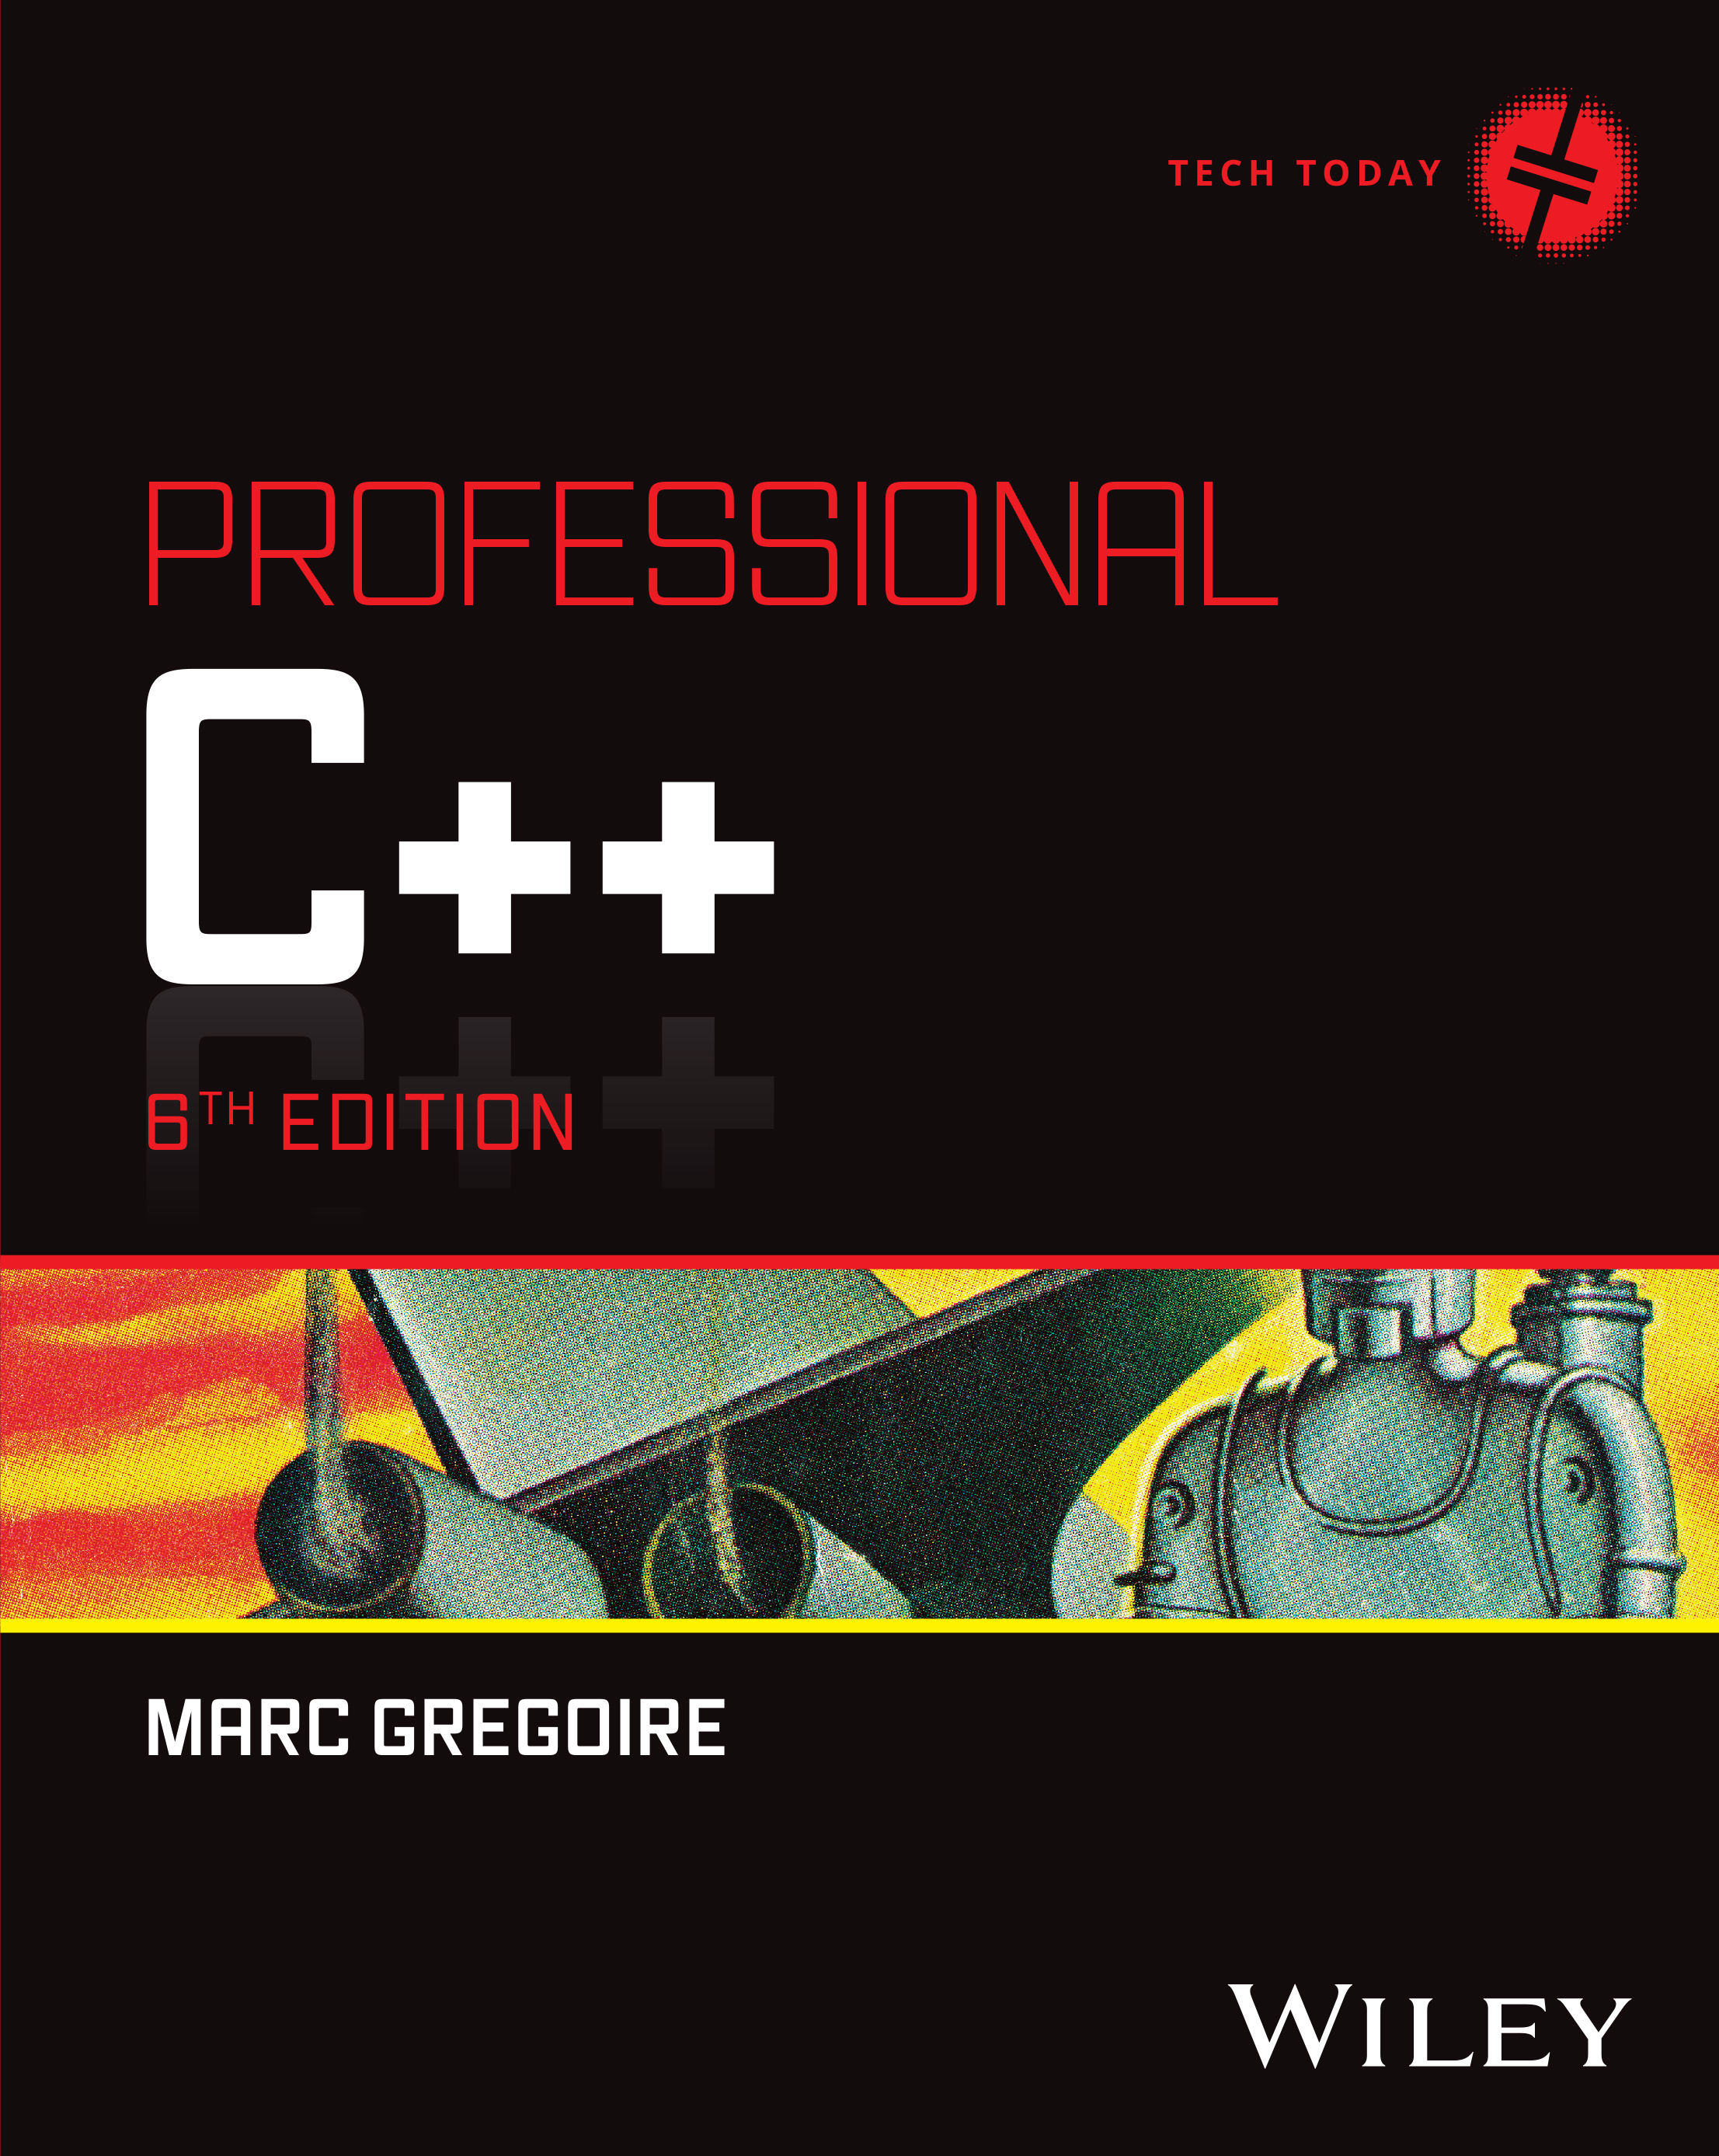
\includegraphics[width=\textwidth,height=\textheight,keepaspectratio]{cover.png}
      \begin{tikzpicture}[remember picture, overlay, inner sep=0pt]
        \node at (current page.center)
        {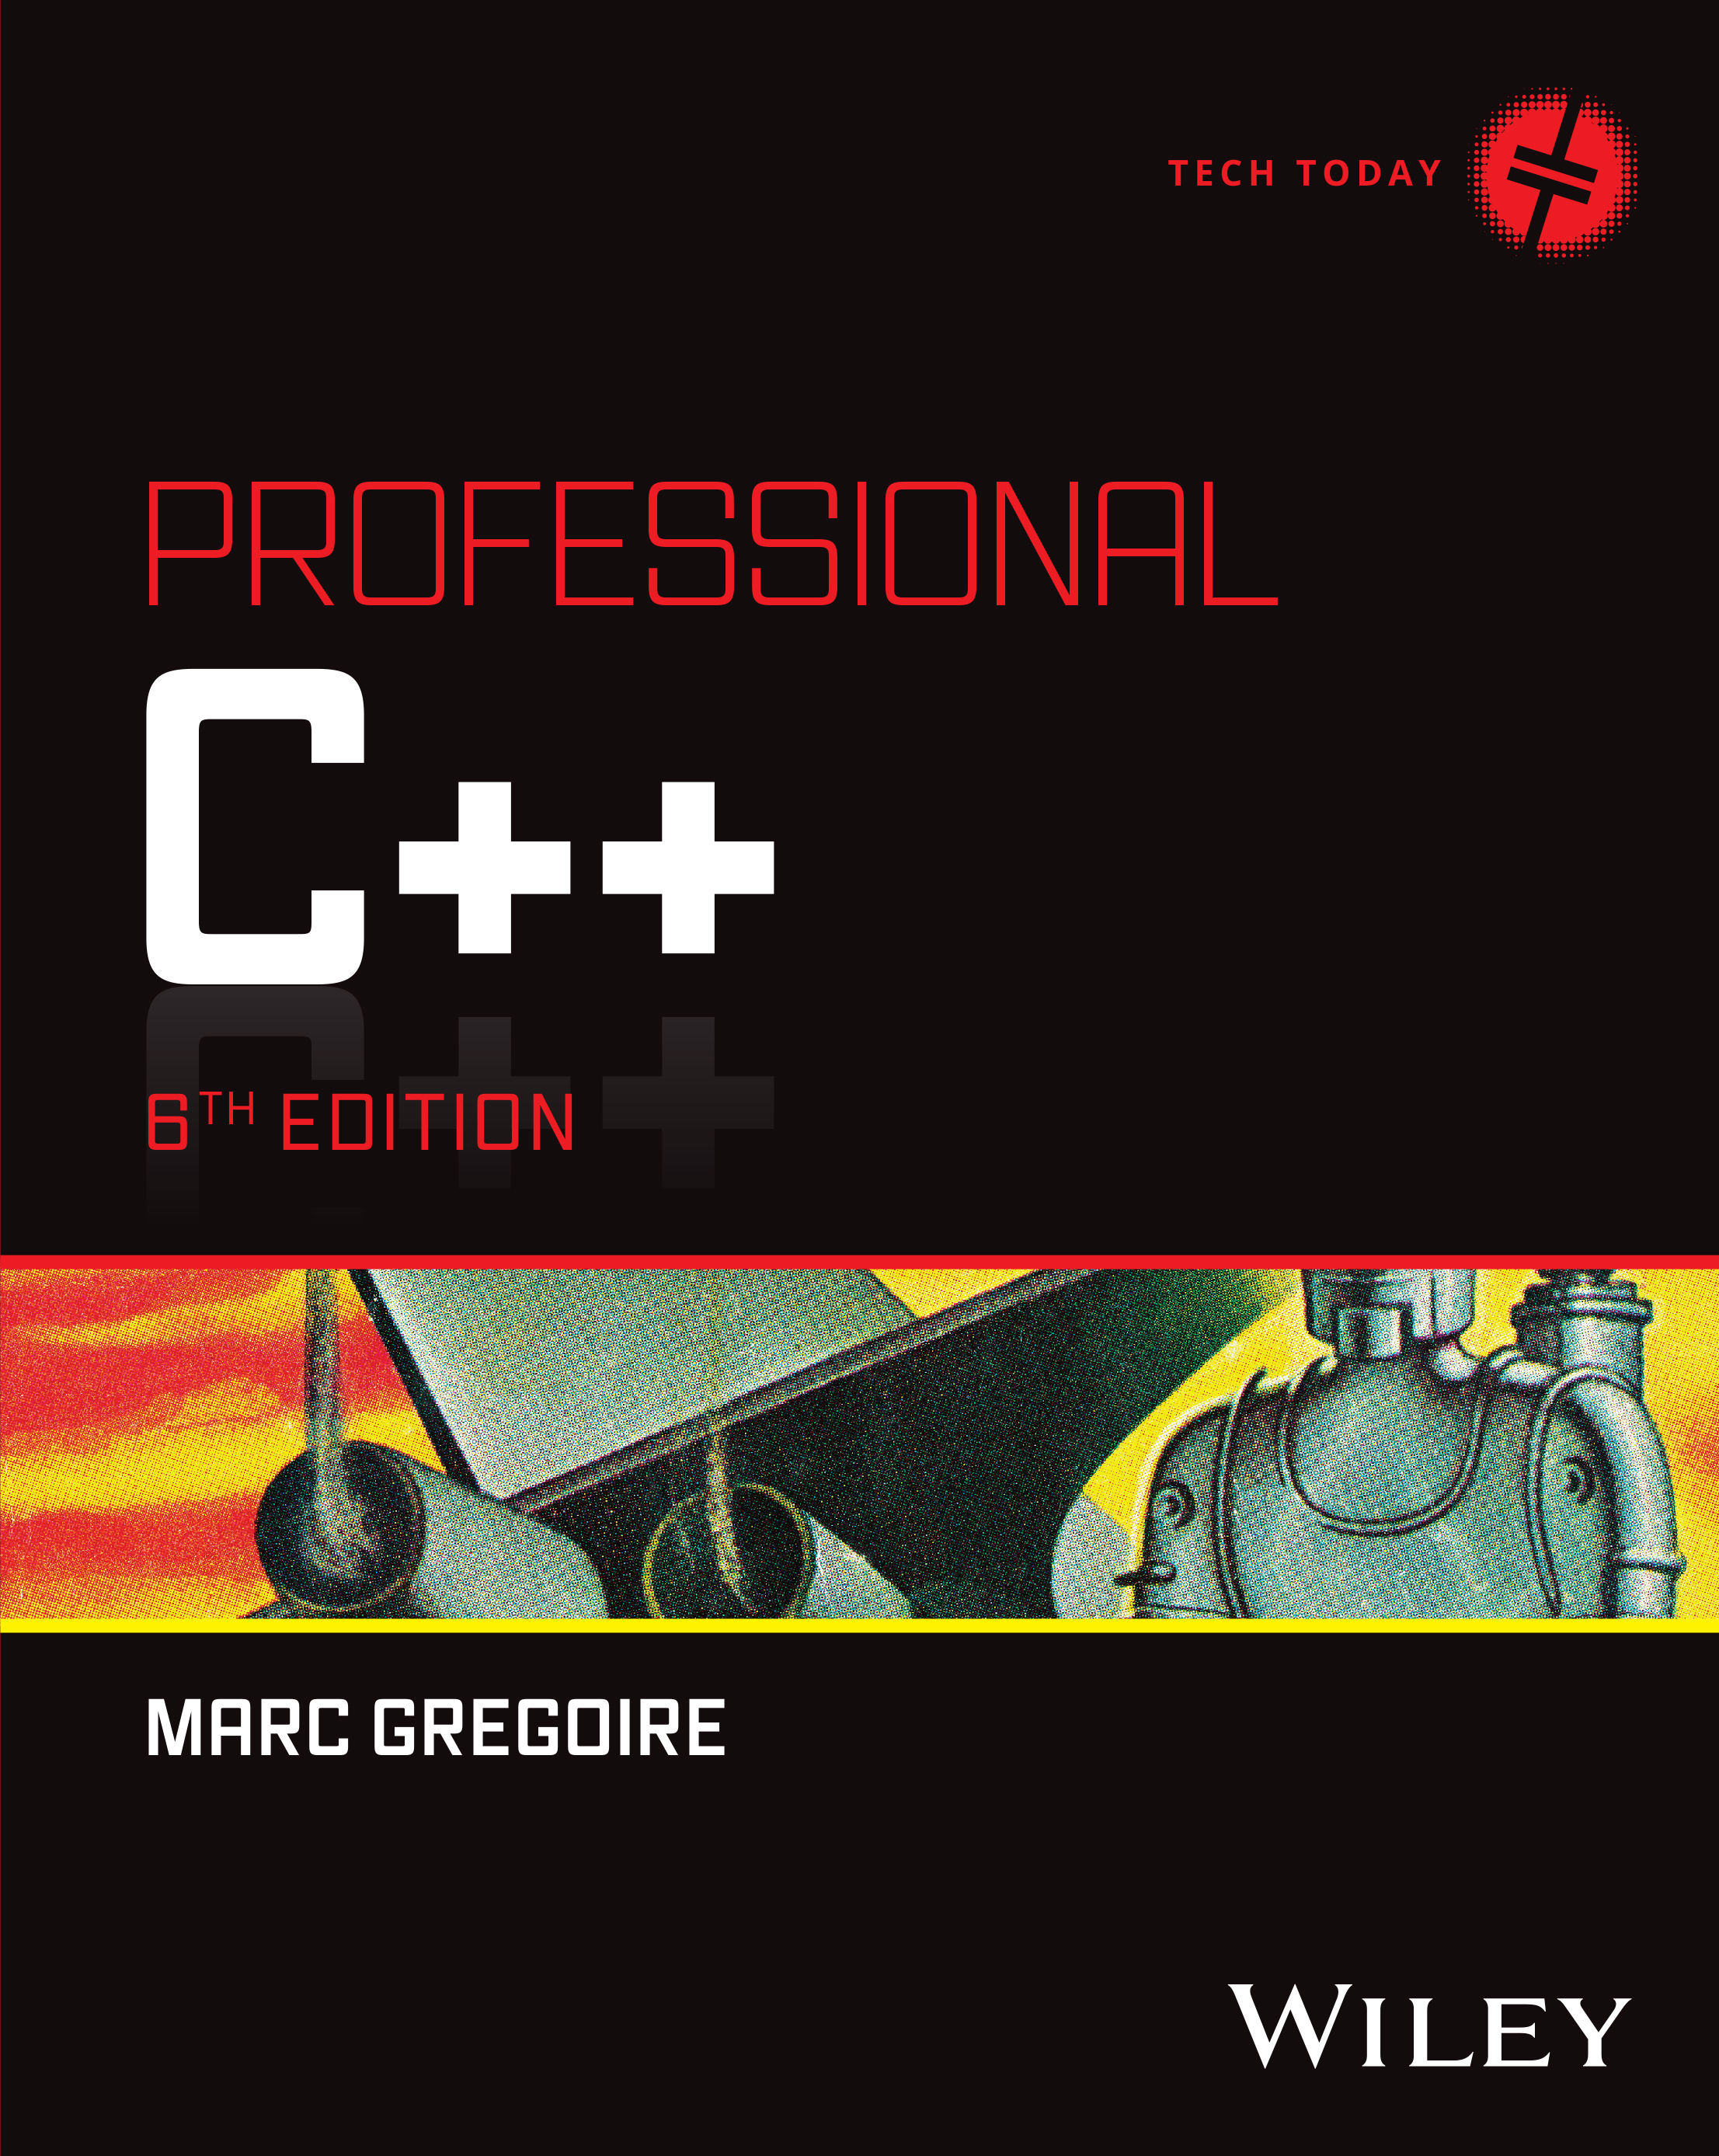
\includegraphics[width=\paperwidth, keepaspectratio=false]{cover.png}};
      \end{tikzpicture}
      \newpage
      \thispagestyle{empty}
      \huge
      \textbf{Learn LLVM 17}
      \\[9pt]
      {\Large 学习LLVM编译器工具和核心库的初学者指南(C++版)}
      \\[9pt]
      \normalsize
      作者: Kai Nacke 和 Amy Kwan
      \\[8pt]
      \normalsize
      译者:\href{https://github.com/xiaoweiChen/The-CXX-Library-Fourth-Edition-include-CXX23}{陈晓伟}
      \\[8pt]
    \end{center}

    \newpage

    \pagestyle{empty}
    \tableofcontents
    \newpage

    \setsecnumdepth{section}

    \textit{
    	\mySection{}{作者致谢}{content/chapter0/0.tex}
    }
    \newpage

    \mySection{}{关于作者}{content/chapter0/1.tex}
    \newpage

    \mySection{}{关于审稿者}{content/chapter0/2.tex}
    \newpage

    \mySection{}{前言}{content/chapter0/3.tex}
    \newpage

    \myPart{第一部分}{使用LLVM构建编译器的基础知识}{content/part1/part1.tex}
    \newpage

    \mySection{第1章}{安装LLVM}{content/part1/chapter1/0.tex}
    \mySubsection{1.1.}{编译与直接安装LLVM}{content/part1/chapter1/1.tex}
    \mySubsection{1.2.}{配置环境}{content/part1/chapter1/2.tex}
    \mySubsection{1.3.}{使用代码库源码进行构建}{content/part1/chapter1/3.tex}
    \mySubsection{1.4.}{自定义构建}{content/part1/chapter1/4.tex}
    \mySubsection{1.5.}{总结}{content/part1/chapter1/5.tex}
    \newpage

    \mySection{第2章}{编译器的结构}{content/part1/chapter2/0.tex}
    \mySubsection{2.1.}{编译器的构建块}{content/part1/chapter2/1.tex}
    \mySubsection{2.2.}{算术表达式语言}{content/part1/chapter2/2.tex}
    \mySubsection{2.3.}{词法分析}{content/part1/chapter2/3.tex}
    \mySubsection{2.4.}{语法分析}{content/part1/chapter2/4.tex}
    \mySubsection{2.5.}{语义分析}{content/part1/chapter2/5.tex}
    \mySubsection{2.6.}{使用LLVM后端生成代码}{content/part1/chapter2/6.tex}
    \mySubsection{2.7.}{总结}{content/part1/chapter2/7.tex}
    \newpage

    \myPart{第二部分}{从源码到机器码}{content/part2/part2.tex}
    \newpage

    \mySection{第3章}{将源码文件转换为抽象语法树}{content/part2/chapter3/0.tex}
    \mySubsection{3.1.}{定义一种编程语言}{content/part2/chapter3/1.tex}
    \mySubsection{3.2.}{项目的目录结构}{content/part2/chapter3/2.tex}
    \mySubsection{3.3.}{管理编译器的输入文件}{content/part2/chapter3/3.tex}
    \mySubsection{3.4.}{处理用户信息}{content/part2/chapter3/4.tex}
    \mySubsection{3.5.}{构造词法分析器}{content/part2/chapter3/5.tex}
    \mySubsection{3.6.}{构建递归下降语法分析器}{content/part2/chapter3/6.tex}
    \mySubsection{3.7.}{执行语义分析}{content/part2/chapter3/7.tex}
    \mySubsection{3.8.}{总结}{content/part2/chapter3/8.tex}
    \newpage

    \mySection{第4章}{生成IR代码的基础知识}{content/part2/chapter4/0.tex}
    \mySubsection{4.1.}{AST生成IR}{content/part2/chapter4/1.tex}
    \mySubsection{4.2.}{使用AST编号生成SSA格式的IR代码}{content/part2/chapter4/2.tex}
    \mySubsection{4.3.}{设置模块和驱动程序}{content/part2/chapter4/3.tex}
    \mySubsection{4.4.}{总结}{content/part2/chapter4/4.tex}
    \newpage

    \mySection{第5章}{高级语言结构生成的IR}{content/part2/chapter5/0.tex}
    \mySubsection{5.1.}{环境要求}{content/part2/chapter5/1.tex}
    \mySubsection{5.2.}{处理数组、结构体和指针}{content/part2/chapter5/2.tex}
    \mySubsection{5.3.}{获得应用程序二进制接口}{content/part2/chapter5/3.tex}
    \mySubsection{5.4.}{为类和虚函数创建IR}{content/part2/chapter5/4.tex}
    \mySubsection{5.5.}{总结}{content/part2/chapter5/5.tex}
    \newpage

    \mySection{第6章}{生成IR代码的进阶知识}{content/part2/chapter6/0.tex}
    \mySubsection{6.1.}{抛出和捕获异常}{content/part2/chapter6/1.tex}
    \mySubsection{6.2.}{为基于类型的别名分析生成元数据}{content/part2/chapter6/2.tex}
    \mySubsection{6.3.}{生成调试元数据}{content/part2/chapter6/3.tex}
    \mySubsection{6.4.}{总结}{content/part2/chapter6/4.tex}
    \newpage

    \mySection{第7章}{优化IR}{content/part2/chapter7/0.tex}
    \mySubsection{7.1.}{环境要求}{content/part2/chapter7/1.tex}
    \mySubsection{7.2.}{LLVM通道管理器}{content/part2/chapter7/2.tex}
    \mySubsection{7.3.}{实现一个新的通道}{content/part2/chapter7/3.tex}
    \mySubsection{7.4.}{使用ppprofiler}{content/part2/chapter7/4.tex}
    \mySubsection{7.5.}{向编译器添加优化管道}{content/part2/chapter7/5.tex}
    \mySubsection{7.6.}{总结}{content/part2/chapter7/6.tex}
    \newpage


    \myPart{第三部分}{LLVM的进阶}{content/part3/part3.tex}
    \newpage

    \mySection{第8章}{TableGen语言}{content/part3/chapter8/0.tex}
    \mySubsection{8.1.}{环境要求}{content/part3/chapter8/1.tex}
    \mySubsection{8.2.}{了解TableGen语言}{content/part3/chapter8/2.tex}
    \mySubsection{8.3.}{实验TableGen语言}{content/part3/chapter8/3.tex}
    \mySubsection{8.4.}{使用TableGen文件生成C++代码}{content/part3/chapter8/4.tex}
    \mySubsection{8.5.}{TableGen的缺点}{content/part3/chapter8/5.tex}
    \mySubsection{8.6.}{总结}{content/part3/chapter8/6.tex}
    \newpage

    \mySection{第9章}{JIT编译}{content/part3/chapter9/0.tex}
    \mySubsection{9.1.}{环境要求}{content/part3/chapter9/1.tex}
    \mySubsection{9.2.}{LLVM的整体JIT的实现和用例}{content/part3/chapter9/2.tex}
    \mySubsection{9.3.}{使用JIT直接执行}{content/part3/chapter9/3.tex}
    \mySubsection{9.4.}{用LLJIT实现JIT编译器}{content/part3/chapter9/4.tex}
    \mySubsection{9.5.}{从头开始构建JIT编译器类}{content/part3/chapter9/5.tex}
    \mySubsection{9.6.}{总结}{content/part3/chapter9/6.tex}
    \newpage

    \mySection{第10章}{使用LLVM工具进行调试}{content/part3/chapter10/0.tex}
    \mySubsection{10.1.}{环境要求}{content/part3/chapter10/1.tex}
    \mySubsection{10.2.}{用消毒器检测应用程序}{content/part3/chapter10/2.tex}
    \mySubsection{10.3.}{使用libFuzzer查找bug}{content/part3/chapter10/3.tex}
    \mySubsection{10.4.}{使用XRay进行性能分析}{content/part3/chapter10/4.tex}
    \mySubsection{10.5.}{使用clang静态分析器检查源代码}{content/part3/chapter10/5.tex}
    \mySubsection{10.6.}{创建基于clang的工具}{content/part3/chapter10/6.tex}
    \mySubsection{10.7.}{总结}{content/part3/chapter10/7.tex}
    \newpage

    \myPart{第四部分}{创建自定义后端}{content/part4/part4.tex}
    \newpage

    \mySection{第11章}{目标描述}{content/part4/chapter11/0.tex}
    \mySubsection{11.1.}{为新后端做准备}{content/part4/chapter11/1.tex}
    \mySubsection{11.2.}{将新架构添加到Triple类中}{content/part4/chapter11/2.tex}
    \mySubsection{11.3.}{扩展LLVM中的ELF文件格式定义}{content/part4/chapter11/3.tex}
    \mySubsection{11.4.}{创建目标描述}{content/part4/chapter11/4.tex}
    \mySubsection{11.5.}{为LLVM添加M88k后端}{content/part4/chapter11/5.tex}
    \mySubsection{11.6.}{实现汇编解析器}{content/part4/chapter11/6.tex}
    \mySubsection{11.7.}{创建反汇编器}{content/part4/chapter11/7.tex}
    \mySubsection{11.8.}{总结}{content/part4/chapter11/8.tex}
    \newpage

    \mySection{第12章}{指令选择}{content/part4/chapter12/0.tex}
    \mySubsection{12.1.}{定义调用约定规则}{content/part4/chapter12/1.tex}
    \mySubsection{12.2.}{通过DAG进行指令选择}{content/part4/chapter12/2.tex}
    \mySubsection{12.3.}{添加寄存器和指令信息}{content/part4/chapter12/3.tex}
    \mySubsection{12.4.}{向下转译空帧}{content/part4/chapter12/4.tex}
    \mySubsection{12.5.}{发出机器指令}{content/part4/chapter12/5.tex}
    \mySubsection{12.6.}{创建目标机器和子目标}{content/part4/chapter12/6.tex}
    \mySubsection{12.7.}{全局指令的选择}{content/part4/chapter12/7.tex}
    \mySubsection{12.8.}{进化后端}{content/part4/chapter12/8.tex}
    \mySubsection{12.9.}{总结}{content/part4/chapter12/9.tex}
    \newpage

    \mySection{第13章}{超越指令选择}{content/part4/chapter13/0.tex}
    \mySubsection{13.1.}{为LLVM添加新机器功能通道}{content/part4/chapter13/1.tex}
    \mySubsection{13.2.}{将新目标集成到clang前端}{content/part4/chapter13/2.tex}
    \mySubsection{13.3.}{针对不同的CPU架构}{content/part4/chapter13/3.tex}
    \mySubsection{13.4.}{总结}{content/part4/chapter13/4.tex}
    \newpage

  \end{sloppypar}
\end{document}

